%!TEX program = xelatex
% Note: this template must be compiled with XeLaTeX rather than PDFLaTeX
% due to the custom fonts used. The line above should ensure this happens
% automatically, but if it doesn't, your LaTeX editor should have a simple toggle
% to switch to using XeLaTeX.

\documentclass[
  aspectratio=169, % Uncomment to use an aspect ratio of 16:9 (160 mm by 90 mm)
  %aspectratio=43, % Uncomment to use an aspect ratio of 4:3 (128mm by 96mm)
  t, % Top align all slide content by default
  onlytextwidth, % Typeset content in columns at text width
  10pt, % Default font size, use 10pt for the 16:9 aspect ratio and 8pt for the 4:3 aspect ratio
]{beamer}

\usepackage{../../ImperialTheme/beamer/beamerthemeImperial} % Use the Imperial theme

\def\imagefolder{../../ImperialTheme/beamer/Images}
\def\Rey{\text{Re}}
\title{Finishing incNS and starting comNS} % Presentation title to appear on the title slide and left footers

\subtitle{} % Presentation subtitle to appear on the title slide

\author{Víctor Ballester} % Author name(s) to appear on the title slide

\date{\today} % Presentation date to appear on the title slide and right footers

\begin{document}

\begingroup
\setbeamercolor{background canvas}{bg=ICLLightGrey} % Slide background color
\setbeamercolor{title page title}{fg=ICLBlue} % Title text color
\setbeamercolor{title page subtitle}{fg=ICLBlue} % Subtitle text color
\setbeamercolor{author}{fg=ICLBlue} % Author(s) text color
\setbeamercolor{date}{fg=ICLBlue} % Date text color
\setbeamertemplate{title page}[logo]{\imagefolder/ICL_Logo_Blue.pdf} % Imperial logo color, use 'ICL_Logo_White.pdf' for white and 'ICL_Logo_Blue.pdf' for blue
\frame[plain, s]{\titlepage} % Output the title page with no footer ('plain') and vertically distributed text ('s')
\endgroup

\begin{frame}
	\frametitle{n-factors}
	\begin{itemize}
		\item Different behaviour in the evolution of the n-factors after the gap. Why? Maybe the unstable frequencies are damp out on the growth in the gap?
	\end{itemize}
	\begin{center}
	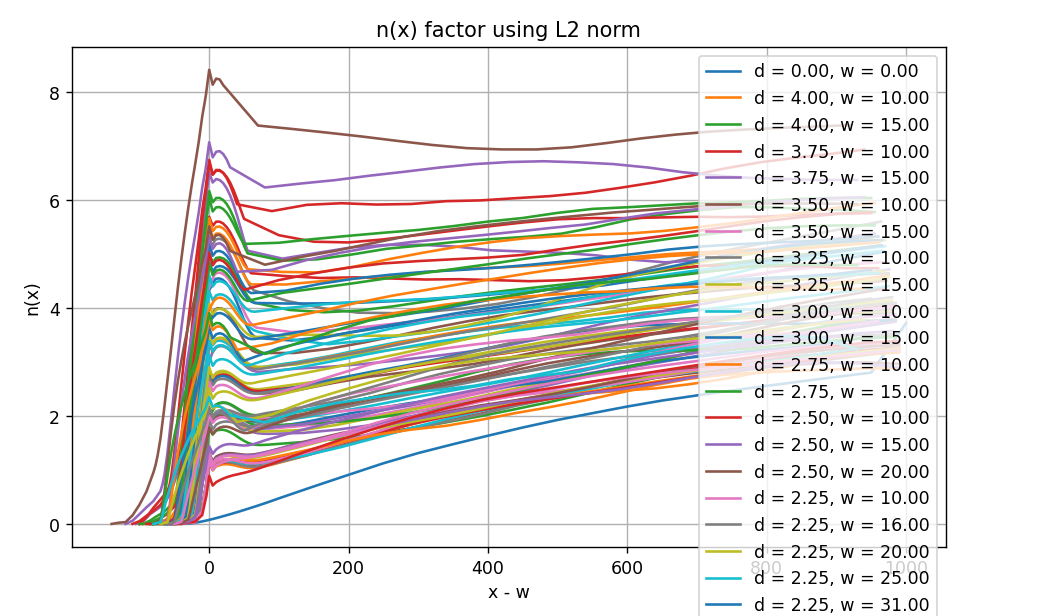
\includegraphics[width=0.65\linewidth]{Images/nfactors.png}
	\end{center}
	
\end{frame}
\begin{frame}
	\frametitle{$\Delta n$-factors}
	\begin{columns}[T] % [T] ensures correct vertical alignment
		\begin{column}{0.38\linewidth} % Left column
			Steps to compute $\Delta n$ (after introducing some noise as body force in the upstream part of the domain):
			\begin{itemize}
			\item $\Delta n$ averaged in the window (gap lies in $x\in(0,w)$): $x\in(w+50,w+250)$.
			\item Cubic interpolation inside the convex hull.
			\item Gaussian filter with $\sigma=2$. Maybe too much? I was getting some weird stripes without filter. 
			\end{itemize}
		\end{column}
		\begin{column}{0.58\linewidth} % Left column
			\begin{center}
				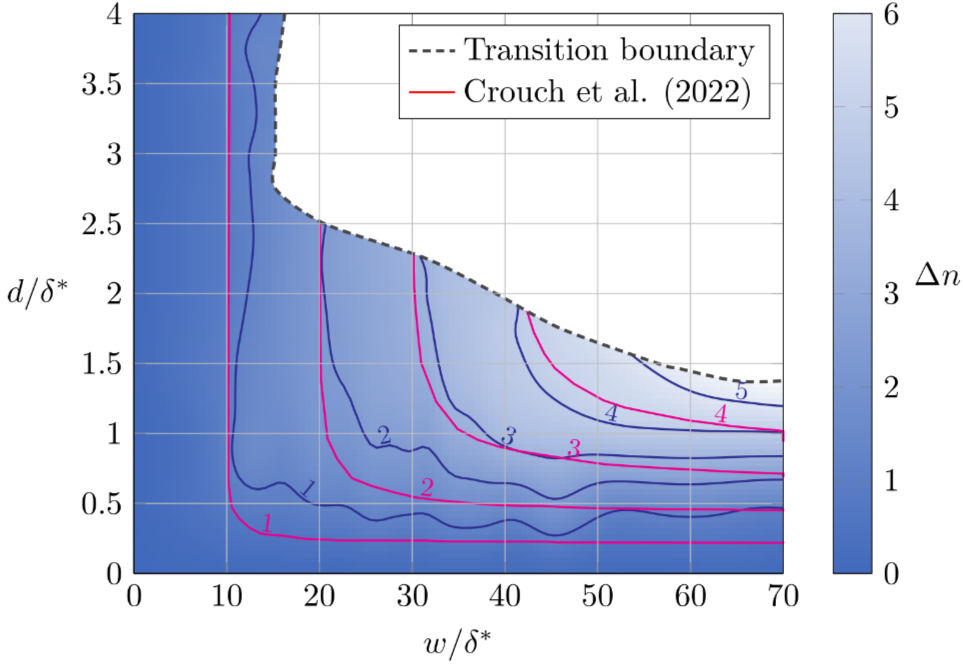
\includegraphics[width=\linewidth]{Images/deltanfactors.png}
			\end{center}
		\end{column}
	\end{columns}
\end{frame}
\begin{frame}
  \frametitle{Compressible Simulations}
  So far they ran, but I had a problem with the blasius that was triggering noise.

  \begin{itemize}
    \item Polynomial order?
    \item CFL?  with the implicit solver. 2 is ok? This translates to $dt \sim 0.06$
  \end{itemize}
  
\end{frame}
\end{document}
